\documentclass[t]{beamer}
\usetheme{Copenhagen}
\setbeamertemplate{headline}{} % remove toc from headers
\beamertemplatenavigationsymbolsempty

\usepackage{amsmath, array, tikz, bm, pgfplots, tcolorbox, graphicx}
\pgfplotsset{compat = 1.16}

\title{Measures of Spread}
\author{}
\date{}

\AtBeginSection[]
{
  \begin{frame}
    \frametitle{Objectives}
    \tableofcontents[currentsection]
  \end{frame}
}

\begin{document}

\begin{frame} 
\maketitle
\end{frame}


\section{Determine the range of a dataset.}

\begin{frame}{The Range}
\begin{tcolorbox}[colframe=green!20!black, colback = green!30!white,title=\textbf{Range}]
The \textbf{range} of a dataset is found by subtracting the minimum value from the maximum value.
\end{tcolorbox}
\end{frame}

\begin{frame}{Example 1}
During a heat wave one summer, I decided to cool off by drinking milkshakes everyday for a week. The number of milkshakes I had each day is shown:	
\begin{center}
9, 2, 7, 10, 3, 4, 12
\end{center}

Find the range for the number of milkshakes I drank that week.	\newline\\
\onslide<2->{Max: 12}	\quad	\onslide<3->{Min: 2}	\newline\\
\onslide<4->{Range: $12-2=10$}
\end{frame}

\begin{frame}{Disadvantage to Using Range to Measure Spread of Data}
A disadvantage of relying solely on the range as a measure of variation is that it is heavily affected by outliers (extreme values).
\end{frame}

\section{Determine the variance and standard deviation of a dataset.}

\begin{frame}{Deviation from Mean}
\begin{tcolorbox}[colframe=green!20!black, colback = green!30!white,title=\textbf{Deviation from the Mean}]
The *\textbf{deviation from the mean} refers to how far a data value, $x$, is from the mean; found by \[x - \text{mean}\].
\end{tcolorbox}
\vspace{11pt}	\pause

A data value that is above the mean has a {\color{blue}\textbf{positive deviation}} and one that is below the mean has a {\color{red}\textbf{negative deviation}}.
\end{frame}

\begin{frame}{Example 2}
Find the mean of the following gas prices: 
\begin{center}
\$3.25, \$3.40, \$3.21, \$3.38
\end{center}
\vspace{8pt}	\pause
Total: \$13.24	\newline\\	\pause
Mean: $\$13.24 / 4 = \$3.31$
\end{frame}

\begin{frame}{Visual Interpretation of the Mean}
We can think of the mean as a ``balancing point'' for our dataset:	\vspace{11pt}
\begin{center}
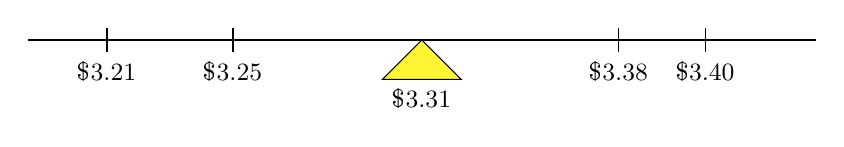
\begin{tikzpicture}
\draw (-5,0) -- (5,0);
\draw [fill=yellow!80] (0,0) -- (-0.5,-0.5) -- (0.5,-0.5) -- cycle;
\node at (0,-0.5) [below] {\small\$3.31};
\draw (-4,0.15) -- (-4,-0.15) node [below] {\small\$3.21};
\draw (-2.4,0.15) -- (-2.4,-0.15) node [below] {\small\$3.25};
\draw (3.6,0.15) -- (3.6,-0.15) node [below] {\small\$3.40};
\draw (2.5,0.15) -- (2.5,-0.15) node [below] {\small\$3.38};
\end{tikzpicture}
\end{center}	\vspace{10pt}	\pause

Each data point has a deviation (or \emph{distance}) from the mean.
\end{frame}

\begin{frame}{Example 3}
Calculate each data point's deviation from the mean.	\newline\\	
\$3.25, \$3.40, \$3.21, \$3.38	\qquad Mean: \$3.31	\newline\\	\pause

\begin{center}
\begin{tabular}{c|c}
\textbf{Price} & \textbf{Deviation from Mean}	\\	\hline
\$3.25			&	$-\$0.06$	\\
\$3.40			&	$\$0.09$	\\
\$3.21			&	$-\$0.10$	\\
\$3.38			&	$\$0.07$	\\
\end{tabular}
\end{center}
\end{frame}

\begin{frame}{Deviations from Mean}
Now, let's get an idea of how much, on average, the data is spread out from the mean.	\newline\\	\pause

We can do that by calculating the mean of the deviations we got in the last example.
\end{frame}

\begin{frame}{Example 4}
Find the mean of the deviations in gas prices from the mean:
\[-\$0.06 \quad \$0.09 \quad -\$0.10 \quad \$0.07\]
\pause
Total: 0	\newline\\	\pause
Mean: $0 / 4 = 0$
\end{frame}

\begin{frame}{Now What?}
It turns out that this will {\color{blue}\textbf{always}} be the case because the total for the positive deviations will always equal the total for negative deviations.	\newline\\	\pause

In order to remedy this issue, of cancelling, we can do one of two things:	\newline\\	\pause

\begin{itemize}
	\item Take the absolute value of the deviations. \newline\\ \pause
	\item Take the squares of the deviations. \newline\\ \pause
\end{itemize}

While the mean of the absolute values of the deviations has its uses (called the \textit{mean absolute deviation}) in terms of calculations, it is better to work with the squares of the deviations instead.
\end{frame}

\begin{frame}{Example 5}
Square each of the deviations in gas prices, then find the mean of the squared deviatons.	\newline\\
\[-\$0.06 \quad \$0.09 \quad -\$0.10 \quad \$0.07	\]	\pause
Squared Deviations:
\[0.0036	\quad 0.0081 \quad 0.01 \quad 0.0049	\]
\pause
Total: 0.0266	\newline\\	\pause
Mean: $0.0266 / 4 = 0.00665$
\end{frame}

\begin{frame}{Population Variance}
The result of the previous example is known as the {\color{blue}\textbf{population variance}} and is denoted by \[\sigma^2\] 
(the lowercase Greek letter sigma, squared).	\newline\\	\pause

Just like mean has a sample mean and a population mean, variance also has a {\color{red}\textbf{sample variance}} and is denoted \[s^2\]
\end{frame}

\begin{frame}{Population Variance vs. Sample Variance}
Sample variance is similar to population variance \emph{except} instead of dividing by the total number of observations, like we did in the gas prices examples, we instead divide by one less than the number of observations (called the {\color{blue}\textbf{degrees of freedom}}).	\newline\\	\pause

Remember, the sum of the deviations from the mean must always equal 0. \newline\\	\pause

In a data set with 4 entries, the first 3 entries can be any number we want (note that $4 - 1 = 3$). The last entry \underline{must} make it so that the sum of the deviations from the mean equals 0.	
\end{frame}

\begin{frame}{Population Variance vs. Sample Variance}
Thus, in a data set with $n$ elements, the first $n-1$ elements can be whatever they want, but that last $n$\textsuperscript{th} element is forced to cause the deviation from the mean to equal 0.	\newline\\	\pause

Another way to describe this difference in denominators is that dividing by $n-1$ does a better job at targeting the actual population variance then dividing by $n$ does when many samples of the population are taken. (Dividing by $n$ under-estimates the population variance).	\newline\\	\pause

Because of this, we say that the sample variance is an {\color{blue}\textbf{unbiased estimator}} of the population variance (that is, the difference between the expected value and the actual value is 0).
\end{frame}


\begin{frame}{Formulas for Population Variance and Sample Variance}
The formulas for population variance and sample variance are below:	\newline\\

\begin{center}
\setlength{\extrarowheight}{7pt}
\begin{tabular}{c|c}
\textbf{Population Variance} & \textbf{Sample Variance} \\ \hline
$\sigma^2 = \frac{\sum (x_i-\mu)^2}{N}$	&	$s^2 = \frac{\sum (x_i-\bar{x})^2}{n-1}$
\end{tabular}
\end{center}
\end{frame}

\begin{frame}{The Units of Measurement with Variance}
The issue with using variance as the primary measure of variation is that variance gives us squared units. The answer to the above example is in square dollars.	\newline\\	\pause

Since we don't normally talk about \emph{squared} dollars, we need to do something to bring those units back down to the same units (dollars) that we started with.	\newline\\	\pause

The {\color{blue}\textbf{standard deviation}} is the square root of the variance: \newline\\ standard deviation = $\sqrt{\text{variance}}$

\[\sigma = \sqrt{\frac{\sum (x_i-\mu)^2}{N}} \quad \text{and} \quad s = \sqrt{\frac{\sum (x_i-\bar{x})^2}{n-1}}\]
\end{frame}

\begin{frame}{Properties of Standard Deviation}
\begin{itemize}
	\item The standard deviation is a measure of how much the data values deviate from the mean.	\newline\\	\pause
	\item The value of the standard deviation can be positive or zero. It can {\color{red}\textbf{never}} be negative.	\newline\\	\pause
	\item The value of the standard deviation can increase dramatically with the inclusion of one or more {\color{blue}\textbf{outliers}} (data values that are very far away from all of the others).	\newline\\	\pause
	\item The units of the standard deviation are the same as the units of the original data values.	\newline\\	\pause
	\item The sample standard deviation, $s$, is a biased estimator of the population standard deviation $\sigma$.	
\end{itemize}
\end{frame}

\begin{frame}{Properties of Standard Deviation}
\begin{itemize}
	\item Population variance = $\sigma^2$	\newline\\	\pause
	\item Sample variance = $s^2$	\newline\\	\pause
	\item Usually, values will be within 2 standard deviations of the mean.
\end{itemize}
\end{frame}

\begin{frame}{Example 6}
The mean price of gas one day was \$3.58 with a standard deviation of \$0.33. What interval would represent a ``usual" price of gas?	\newline\\	\pause

Min price: $3.58 - 2(0.33) = 2.92$	\newline\\	\pause
Max price: $3.58 + 2(0.33) = 4.24$	\newline\\	\pause

The ``usual" price of gas is between \$2.92 and \$4.24.
\end{frame}



\end{document}